% !TEX root = ../main.tex
\chapter{RL Elements and Multi-Armed Bandits}

\section{The RL Elements}
\subsection{Reward}
A reward $R_t$ is a scalar feedback that indicates how well the agent is doing at step $t$.
Step $t$ indicates a discrete time-step (a continuous-time treatment is possible but not considered in this course).
We consider a time-step in:
\begin{enumerate}
    \item \textbf{Episodic tasks:} last for a finite amount of time;
    \item \textbf{Continuing tasks:} never end and continue indefinitely.
\end{enumerate}
The agent's job is to maximize the \textit{cumulative reward}:
\begin{enumerate}
    \item In episodic tasks, cumulative reward over an episode;
    \item In continuing tasks, cumulative reward over a defined horizon (that can be rolling).
\end{enumerate}
RL is based on the \textit{reward hypothesis}:
\begin{center}
  \itshape ``All goals can be described by the maximization of expected cumulative reward.''
\end{center}
Actions may have long-term consequences and rewards may be delayed: immediate rewards can be sacrificed to gain more long term rewards.

\subsection{The Agent and the Environment}
At each step $t$ the agent is in the state $S_t$ and takes an action $A_t$ that is a feasible action from that state. The environment, based on the state-action pair $(S_t, A_t)$, returns a reward $R_{t+1}$ and moves the agent in the state $S_{t+1}$.

\subsection{Observation and History}
Moreover, at each step the agent sees an \textit{observation} $O_{t+1}$:
\begin{itemize}
    \item In \textit{fully observable environments} $S_{t+1}=O_{t+1}$;
    \item In \textit{partially observable environments} the state is not available and must be inferred from the history:
    \[H_t=O_1,R_1,A_1,...,A_{t-1},O_t,R_t\]\[S_t=f(H_t)\] 
\end{itemize}
If we can't have a reliable state we must define different strategies (taking whole history as state or estimate the state with a supervised learning approximation).

\subsection{Components of an Agent}
An agent may have the following components:
\begin{itemize}
    \item (always) a \textit{policy}, the function that describes the behavior of the agent and maps states to actions. The RL goal is to find the optimal policy. Policy can be:
        \begin{itemize}
            \item \textit{Deterministic policy}, $a=\pi(s)$
            \item \textit{Stochastic policy}, $\pi(a|s)=P[A_t=a|S_t=s]$
        \end{itemize}
    \item (possibly) a \textit{value function}, a quantitative description of how good each state is;
    \item (possibly) a \textit{q-value function}, a quantitative description of how good a (state,action) pair is;
    \item (possibly) a \textit{model}, the agent's representation of the environment.
\end{itemize}

\section{Multi-armed Bandits}
In this case we consider simple settings where there is only one state ($S_t=S_{t+1}$) and the agent has to choose among $k$ actions (arms of a bandit). The agent's goal is to maximize the expected reward over time. The agent must balance exploration (trying new actions) and exploitation (choosing the best-known action).

In the example of slot machines (`one-armed bandits'), each machine is associated with a different probability distribution of rewards. At each episode the agent can pull only one lever. The aim is to understand the best strategy to maximize cumulative rewards over different episodes. 

\subsection{Action Values}
Each action provides a stochastic reward, and the q-value of an action is the following (we are considering that the state never changes):
\[q_*(a)\doteq\mathbb{E}[R_t\mid A_t=a]\]
In this case $t$ indicates the episode number, while in typical RL settings it indicates the time-step within an episode.

The q-value for an action is not known and must be estimated, a simple way is by the \textit{Sample-Average} method:
\[Q_t(a)\doteq\frac{\text{sum of rewards when }a\text{ is taken prior to }t}{\text{number of times }a\text{ is taken prior to }t}=\frac{\sum_{i=1}^{t-1}R_i\cdot\mathds{1}_{A_i=a}}{\sum_{i=1}^{t-1}\mathds{1}_{A_i=a}}\]
where $\mathds{1}_{\text{predicate}}$ equals 1 if the predicate is true and 0 otherwise. Every time I collect a new data point I can recompute this estimate.

\subsection{Incremental Implementation of Action Value Estimate}
If we consider a single action $a$ and $R_i$ the reward received after the $i$-th selection of $a$, after $n-1$ selections of action $a$ we can estimate its action value as:
\[Q_n\doteq\frac{R_1+R_2+\cdots{}+R_{n-1}}{n-1}\]
This approach is not efficient because memory and computation will grow over time.
\begin{equation}
\begin{split}
  Q_{n+1}&=\frac{1}{n}\sum_{i=1}^{n}R_i \\
  &=\frac{1}{n}\left(R_n+\sum_{i=1}^{n-1}R_i\right) \\
  &=\frac{1}{n}\left(R_n+(n-1)Q_n\right) \\
  &=\frac{1}{n}\left(R_n+nQ_n-Q_n\right) \\
  &=Q_n+\frac{1}{n}\left(R_n-Q_n\right)
\end{split}
\end{equation}
This implementation requires only $Q_n$ and $n$ to compute $Q_{n+1}$, we don't need all the past values of the rewards.
The more rewards I see, the less relevant the `innovation' is (not ideal for non-stationary problems).
For this reason we move to a step-size that does not change over time (typically $\alpha\in(0,1]$).
\[\textit{NewEstimate}\leftarrow\textit{OldEstimate}+\textit{StepSize}\left[\textit{Target}-\textit{OldEstimate}\right]\]
In this way I also don't need to keep track of the number of times an action has been selected, but I need to choose a step-size $\alpha$. The result is an \textit{exponential recency-weighted average}, which gradually forgets old rewards. This is convenient for \textit{non-stationary} problems where the reward distribution of the actions changes over time.
\begin{equation}
\begin{split}
  Q_{n+1}&=Q_n+\alpha\left(R_n-Q_n\right) \\
  &=\alpha R_n+(1-\alpha)Q_n \\
  &=\alpha R_n+(1-\alpha)\left[\alpha R_{n-1}+(1-\alpha)Q_{n-1}\right] \\
  &=\alpha R_n+\alpha(1-\alpha)R_{n-1}+(1-\alpha)^2Q_{n-1} \\
  &=\alpha R_n+\alpha(1-\alpha)R_{n-1}+\alpha(1-\alpha)^2R_{n-2}+ \\ &\cdots{}+\alpha(1-\alpha)^{n-1}R_1+(1-\alpha)^nQ_1 \\
  &=(1-\alpha)^nQ_1+\sum_{i=1}^{n}\alpha(1-\alpha)^{n-i}R_i
\end{split}
\end{equation}
\subsection{Greedy Policy}
With a greedy policy the selected action will be:
\[A_t\doteq\argmax_{a}Q_t(a)\]
This policy is the simplest one, but it does not explore: we may get stuck with a suboptimal action.

\subsection{Exploration vs Exploitation}
\textit{Exploration} allows us to improve knowledge for long-term benefit, while \textit{Exploitation} exploits knowledge for short-term benefit.
We cannot explore and exploit at the same time, so implementing a trade-off is necessary to avoid suboptimal solutions. There are different approaches to cope with the trade-off:
\begin{itemize}
    \item $\varepsilon$-greedy;
    \item greedy with optimistic initialization;
    \item Upper Confidence Bound (UCB);
    \item Gradient Bandit.
\end{itemize}

\subsubsection{\texorpdfstring{$\boldsymbol{\varepsilon}$}{epsilon}-Greedy Policy}
This is a stochastic policy, defined as follows:
\begin{equation}
  A_t\overset{\text{def}}{=}
  \begin{cases}
    \text{greedy action with probability }1-\varepsilon\\
    \text{a random action among all }k\text{ with probability } \varepsilon
  \end{cases}
\end{equation}
with $\varepsilon\in(0,1)$ (typically a small number). In the random case the action is chosen uniformly among all $k$, including the greedy one.

\begin{esempio}{The 10-armed testbed}
Consider \textbf{2000 randomly generated} 10-armed bandit problems.

\medskip
\noindent\textbf{Generating a problem.}
For each problem, the true action values are drawn as
$q_*(a) \sim \mathcal{N}(0,1)$ for $a = 1,\dots,10$.
When the agent selects action $a$, it receives
$R \sim \mathcal{N}(q_*(a),\,1)$.

\medskip
\noindent\textbf{What the agent does.}
In each problem the agent starts with all estimates set to zero and plays
$1000$ steps, updating $Q_t(a)$ along the way. There is no memory
between one problem and the next (independent problems).

\medskip
\noindent\textbf{Evaluation.}
At each step $t$, performance is averaged over the 2000 problems:
\[
  \bar{R}_t = \frac{1}{2000}\sum_{k=1}^{2000} R_t^{(k)}
  \qquad
  \%\text{ optimal}_t = \frac{1}{2000}\sum_{k=1}^{2000}
  \mathds{1}_{A_t^{(k)} = \arg\max_a q_*^{(k)}(a)}
\]
\begin{center}
  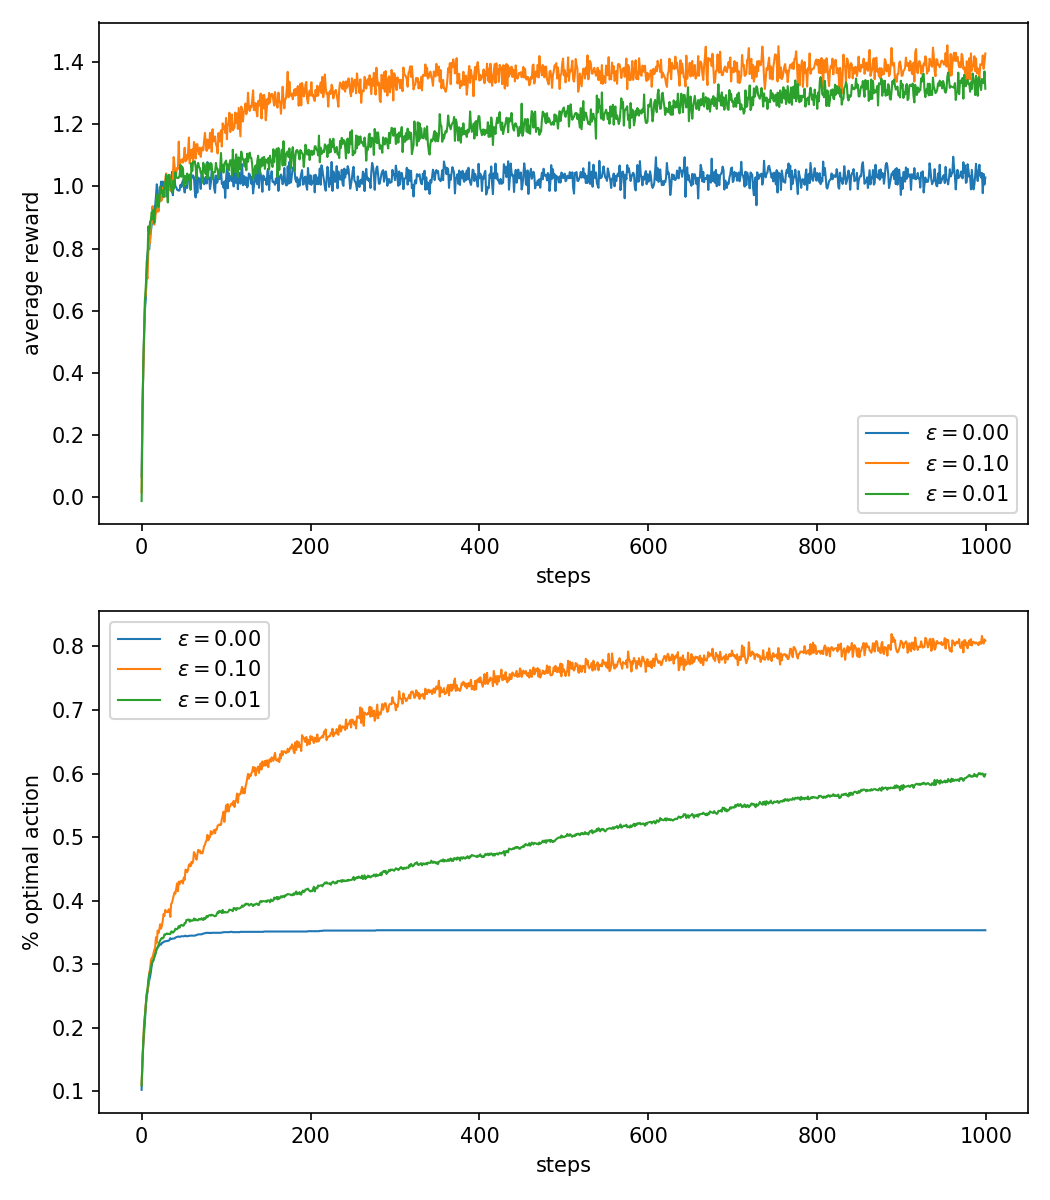
\includegraphics[width=0.85\linewidth]{./figures/chapter2/bandit_testbed.png}
  \captionof{figure}{Comparison of $\varepsilon$-greedy policies on the 10-armed testbed, averaged over 2000 randomly generated problems, each played for 1000 steps.}
  \label{fig:testbed}
\end{center}
The best value of $\varepsilon$ depends on the problem: with noisier rewards more exploration would help, and in longer runs $\varepsilon=0.01$ eventually outperforms $\varepsilon=0.1$.
\end{esempio} 

\begin{algobox}{A simple bandit algorithm}
Initialize, for $a = 1$ to $k$:\\
\hspace*{1.5em}$Q(a) \leftarrow 0$\\
\hspace*{1.5em}$N(a) \leftarrow 0$

\medskip
Loop forever:\\
\hspace*{1.5em}$A \leftarrow
\begin{cases}
  \argmax_a Q(a) & \text{with probability } 1-\varepsilon \\
  \text{a random action} & \text{with probability } \varepsilon
\end{cases}$\\[2pt]
\hspace*{1.5em}$R \leftarrow \mathit{bandit}(A)$\\
\hspace*{1.5em}$N(A) \leftarrow N(A) + 1$\\
\hspace*{1.5em}$Q(A) \leftarrow Q(A) + \frac{1}{N(A)}\bigl[R - Q(A)\bigr]$
\end{algobox}

\subsubsection{Greedy with Optimistic Initialization}
We can initialize the action-value estimates to a high value, this will encourage exploration in the early stages of learning (`optimism in the face of uncertainty'): whatever action is selected, the reward is lower than the estimate, so the agent is `disappointed' and tries the other actions.
The only difference in the algorithm is the initialization of the action-value estimates, which are set to a high value instead of zero ($Q(a)\leftarrow Q_0$). However, it has some limitations:
\begin{itemize}
    \item it only drives early exploration, so it is not well-suited for non-stationary problems;
    \item in some applications we may not know what an optimistic initial value should be.
\end{itemize}
Anyway, it is a convenient heuristic, typically combined with other approaches (e.g., optimistic initialization + $\varepsilon$-greedy).

\subsubsection{Upper-Confidence-Bound (UCB)}
\textit{UCB} uses uncertainty in the value estimates to balance exploration and exploitation. The action selection is based on the following formula:
\[A_t\doteq\argmax_a \left[Q_t(a) + c\sqrt{\frac{\ln t}{N_t(a)}}\right]\]
where $N_t(a)$ is the number of times action $a$ has been selected prior to time $t$ (if $N_t(a)=0$, $a$ is considered a maximizing action). The exploration term comes from \textit{Hoeffding's inequality}. Note that the confidence interval is on our estimate $Q_t(a)$, not on the reward distribution. The more we take an action, the narrower the confidence interval becomes, and the less we explore that action. The parameter $c$ controls the degree of exploration. In a sense, we take the action that potentially could be the best, considering both the estimated value and the uncertainty in that estimate.
\begin{figure}[H]
  \centering
  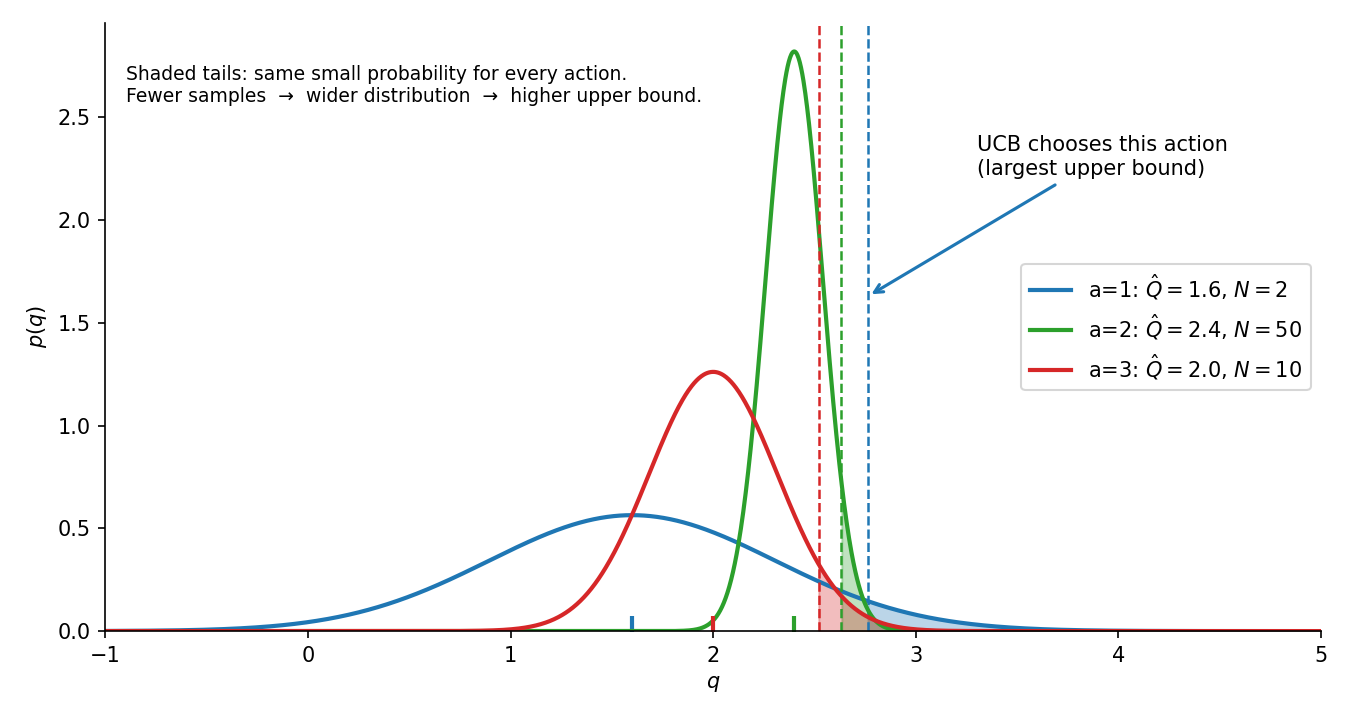
\includegraphics[width=0.9\textwidth]{figures/chapter2/hoeffding_ucb.png}
  \caption{Intuition behind UCB via Hoeffding's inequality. Each curve represents
  the uncertainty about $q_*(a)$; the dashed lines are the upper bounds
  $Q_t(a) + U_t(a)$, chosen so that the shaded tails have the same small
  probability. The least explored action ($N=2$) has the largest bound and is
  selected.}
  \label{fig:hoeffding-ucb}
\end{figure}

\subsubsection{Gradient Bandit Algorithms (GBA)}
In \textit{GBA} a preference for each action is defined $H_t(a)\in\R$, the larger the preference, the more often the action is taken. Preferences have no interpretation in terms of reward: only the relative preference of one action over another matters. The action selection is based on a softmax distribution:
\[\Pr\{A_t=a\}\doteq\frac{e^{H_t(a)}}{\sum_{b=1}^k e^{H_t(b)}}\doteq\pi_t(a)\]
where $\pi_t(a)$ is the probability of taking action $a$ at time $t$. Initially all preferences are equal (e.g., $H_1(a)=0$ for all $a$).
The Gradient Bandit Algorithm updates action preferences using
gradient ascent on the expected reward:

\[
H_{t+1}(a) = H_t(a) +
\alpha (R_t - \bar{R}_t)
\frac{\partial \ln \pi_t(A_t)}{\partial H_t(a)}
\]

Given the softmax policy:

\[
\pi_t(a) =
\frac{e^{H_t(a)}}{\sum_{b=1}^{k} e^{H_t(b)}}
\]

Taking its logarithm:

\[
\ln \pi_t(A_t)
= H_t(A_t) -
\ln \left( \sum_{b=1}^{k} e^{H_t(b)} \right)
\]

The derivative depends on whether the action is selected:

\[
\frac{\partial \ln \pi_t(A_t)}{\partial H_t(a)}
=
\begin{cases}
1 - \pi_t(A_t), & a = A_t \\[4pt]
-\pi_t(a), & a \neq A_t
\end{cases}
\]

that is, $\frac{\partial \ln \pi_t(A_t)}{\partial H_t(a)}=\mathds{1}_{a=A_t}-\pi_t(a)$. Therefore, the two update rules follow directly from
the gradient of the log-softmax policy (the full derivation as stochastic gradient ascent is in the book and is not exam material):

\[H_{t+1}(A_t)\doteq H_t(A_t)+\alpha(R_t-\bar{R}_t)(1-\pi_t(A_t))\]
and for all $a\ne A_t$:
\[H_{t+1}(a)\doteq H_t(a)-\alpha(R_t-\bar{R}_t)\pi_t(a)\]
with $\alpha$ the step-size parameter and $\bar{R}_t$ the average of the rewards up to but not including time $t$, which works as a \textit{baseline}. The update rule increases the preference for the selected action if the received reward is greater than the average reward, and decreases it otherwise.
Higher $\alpha$ causes faster updates, making the policy more deterministic (more Exploitation). A low $\alpha$ causes slower updates, making the policy more stochastic (more Exploration).

\subsection{Summary: comparing exploration strategies}

To compare the methods, each algorithm was run on the 10-armed testbed
for different values of its own parameter, measuring the average reward
over the first 1000 steps (\cref{fig:parameter-study}).

\begin{figure}[H]
  \centering
  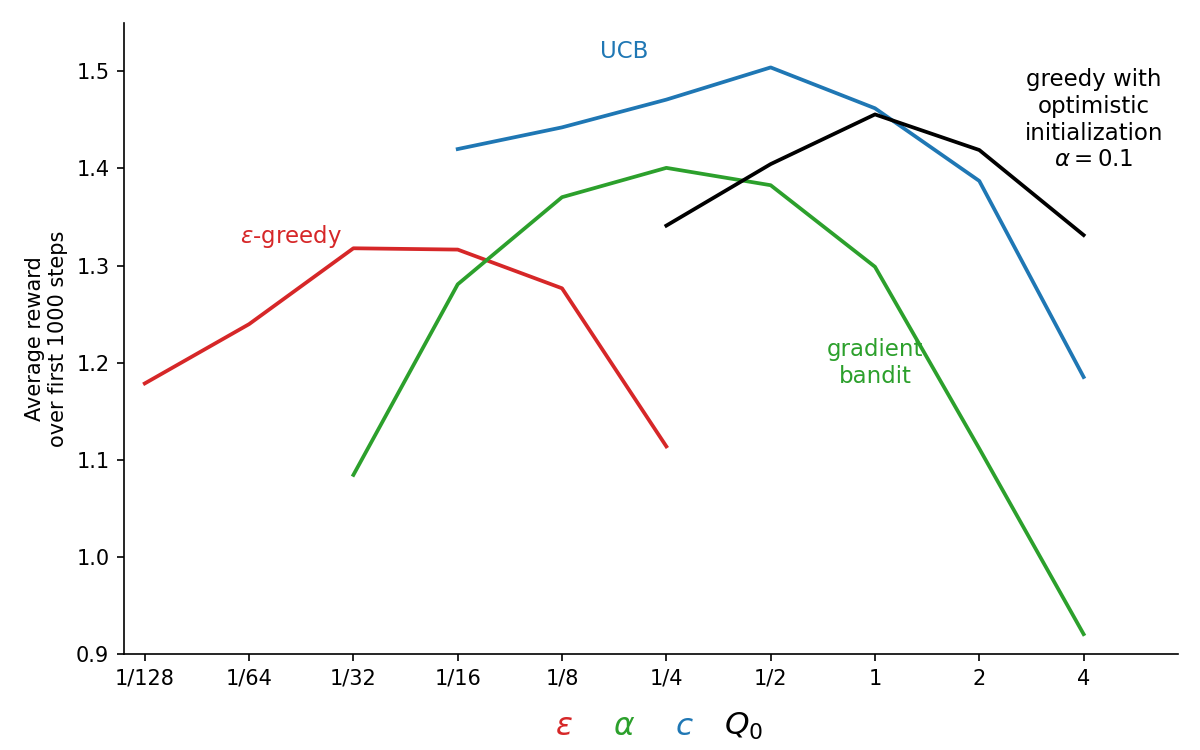
\includegraphics[width=0.85\textwidth]{figures/chapter2/parameter_study.png}
  \caption{Parameter study on the 10-armed testbed: average reward over the first 1000 steps of each algorithm, as a function of its parameter ($\varepsilon$, $\alpha$, $c$ or $Q_0$).}
  \label{fig:parameter-study}
\end{figure}
There is always a trade-off in the choice of the parameter, related to the exploration--exploitation trade-off. The result depends on the problem and on the number of steps
available: with a different horizon, or a non-stationary
problem, the ranking and the best parameters may change a lot.

Topics not covered here: the concept of \textit{regret} (the missed opportunity with respect to always playing the best action) and \textit{contextual bandits} (bandits with states, e.g., using information about the user in advertising).

\section{What Really Matters: Rewards, Not Estimates}
In RL we do not try to model the full reward distributions: it would be too
data-expensive and unnecessary, since our goal is only to maximize the reward
(\emph{``All models are wrong, but some are useful''}, G.~Box). For the same reason, we do not need our estimates $Q(a)$ to be close to the
true values $q_*(a)$. What matters is that they lead us to choose the right
action. A policy is evaluated by the rewards it collects, not by how accurate
its estimates are: estimates that are far from the true values, but still
identify the best action are more useful than estimates that are closer on
average but point to the wrong action.
